% Options for packages loaded elsewhere
\PassOptionsToPackage{unicode}{hyperref}
\PassOptionsToPackage{hyphens}{url}
%
\documentclass[
]{article}
\usepackage{amsmath,amssymb}
\usepackage{lmodern}
\usepackage{iftex}
\ifPDFTeX
  \usepackage[T1]{fontenc}
  \usepackage[utf8]{inputenc}
  \usepackage{textcomp} % provide euro and other symbols
\else % if luatex or xetex
  \usepackage{unicode-math}
  \defaultfontfeatures{Scale=MatchLowercase}
  \defaultfontfeatures[\rmfamily]{Ligatures=TeX,Scale=1}
\fi
% Use upquote if available, for straight quotes in verbatim environments
\IfFileExists{upquote.sty}{\usepackage{upquote}}{}
\IfFileExists{microtype.sty}{% use microtype if available
  \usepackage[]{microtype}
  \UseMicrotypeSet[protrusion]{basicmath} % disable protrusion for tt fonts
}{}
\makeatletter
\@ifundefined{KOMAClassName}{% if non-KOMA class
  \IfFileExists{parskip.sty}{%
    \usepackage{parskip}
  }{% else
    \setlength{\parindent}{0pt}
    \setlength{\parskip}{6pt plus 2pt minus 1pt}}
}{% if KOMA class
  \KOMAoptions{parskip=half}}
\makeatother
\usepackage{xcolor}
\IfFileExists{xurl.sty}{\usepackage{xurl}}{} % add URL line breaks if available
\IfFileExists{bookmark.sty}{\usepackage{bookmark}}{\usepackage{hyperref}}
\hypersetup{
  pdftitle={Topic 04 - Sentiment Analysis II},
  pdfauthor={Julia Parish},
  hidelinks,
  pdfcreator={LaTeX via pandoc}}
\urlstyle{same} % disable monospaced font for URLs
\usepackage[margin=1in]{geometry}
\usepackage{color}
\usepackage{fancyvrb}
\newcommand{\VerbBar}{|}
\newcommand{\VERB}{\Verb[commandchars=\\\{\}]}
\DefineVerbatimEnvironment{Highlighting}{Verbatim}{commandchars=\\\{\}}
% Add ',fontsize=\small' for more characters per line
\usepackage{framed}
\definecolor{shadecolor}{RGB}{248,248,248}
\newenvironment{Shaded}{\begin{snugshade}}{\end{snugshade}}
\newcommand{\AlertTok}[1]{\textcolor[rgb]{0.94,0.16,0.16}{#1}}
\newcommand{\AnnotationTok}[1]{\textcolor[rgb]{0.56,0.35,0.01}{\textbf{\textit{#1}}}}
\newcommand{\AttributeTok}[1]{\textcolor[rgb]{0.77,0.63,0.00}{#1}}
\newcommand{\BaseNTok}[1]{\textcolor[rgb]{0.00,0.00,0.81}{#1}}
\newcommand{\BuiltInTok}[1]{#1}
\newcommand{\CharTok}[1]{\textcolor[rgb]{0.31,0.60,0.02}{#1}}
\newcommand{\CommentTok}[1]{\textcolor[rgb]{0.56,0.35,0.01}{\textit{#1}}}
\newcommand{\CommentVarTok}[1]{\textcolor[rgb]{0.56,0.35,0.01}{\textbf{\textit{#1}}}}
\newcommand{\ConstantTok}[1]{\textcolor[rgb]{0.00,0.00,0.00}{#1}}
\newcommand{\ControlFlowTok}[1]{\textcolor[rgb]{0.13,0.29,0.53}{\textbf{#1}}}
\newcommand{\DataTypeTok}[1]{\textcolor[rgb]{0.13,0.29,0.53}{#1}}
\newcommand{\DecValTok}[1]{\textcolor[rgb]{0.00,0.00,0.81}{#1}}
\newcommand{\DocumentationTok}[1]{\textcolor[rgb]{0.56,0.35,0.01}{\textbf{\textit{#1}}}}
\newcommand{\ErrorTok}[1]{\textcolor[rgb]{0.64,0.00,0.00}{\textbf{#1}}}
\newcommand{\ExtensionTok}[1]{#1}
\newcommand{\FloatTok}[1]{\textcolor[rgb]{0.00,0.00,0.81}{#1}}
\newcommand{\FunctionTok}[1]{\textcolor[rgb]{0.00,0.00,0.00}{#1}}
\newcommand{\ImportTok}[1]{#1}
\newcommand{\InformationTok}[1]{\textcolor[rgb]{0.56,0.35,0.01}{\textbf{\textit{#1}}}}
\newcommand{\KeywordTok}[1]{\textcolor[rgb]{0.13,0.29,0.53}{\textbf{#1}}}
\newcommand{\NormalTok}[1]{#1}
\newcommand{\OperatorTok}[1]{\textcolor[rgb]{0.81,0.36,0.00}{\textbf{#1}}}
\newcommand{\OtherTok}[1]{\textcolor[rgb]{0.56,0.35,0.01}{#1}}
\newcommand{\PreprocessorTok}[1]{\textcolor[rgb]{0.56,0.35,0.01}{\textit{#1}}}
\newcommand{\RegionMarkerTok}[1]{#1}
\newcommand{\SpecialCharTok}[1]{\textcolor[rgb]{0.00,0.00,0.00}{#1}}
\newcommand{\SpecialStringTok}[1]{\textcolor[rgb]{0.31,0.60,0.02}{#1}}
\newcommand{\StringTok}[1]{\textcolor[rgb]{0.31,0.60,0.02}{#1}}
\newcommand{\VariableTok}[1]{\textcolor[rgb]{0.00,0.00,0.00}{#1}}
\newcommand{\VerbatimStringTok}[1]{\textcolor[rgb]{0.31,0.60,0.02}{#1}}
\newcommand{\WarningTok}[1]{\textcolor[rgb]{0.56,0.35,0.01}{\textbf{\textit{#1}}}}
\usepackage{graphicx}
\makeatletter
\def\maxwidth{\ifdim\Gin@nat@width>\linewidth\linewidth\else\Gin@nat@width\fi}
\def\maxheight{\ifdim\Gin@nat@height>\textheight\textheight\else\Gin@nat@height\fi}
\makeatother
% Scale images if necessary, so that they will not overflow the page
% margins by default, and it is still possible to overwrite the defaults
% using explicit options in \includegraphics[width, height, ...]{}
\setkeys{Gin}{width=\maxwidth,height=\maxheight,keepaspectratio}
% Set default figure placement to htbp
\makeatletter
\def\fps@figure{htbp}
\makeatother
\setlength{\emergencystretch}{3em} % prevent overfull lines
\providecommand{\tightlist}{%
  \setlength{\itemsep}{0pt}\setlength{\parskip}{0pt}}
\setcounter{secnumdepth}{-\maxdimen} % remove section numbering
\setlength{\parindent}{1em}
\usepackage{float}
\ifLuaTeX
  \usepackage{selnolig}  % disable illegal ligatures
\fi

\title{Topic 04 - Sentiment Analysis II}
\author{Julia Parish}
\date{2022-04-26}

\begin{document}
\maketitle

\hypertarget{sentiment-analyis-ii}{%
\section{Sentiment Analyis II}\label{sentiment-analyis-ii}}

This text sentiment analysis was completed as an assignment for the
course, Environmental Data Science 231: Text and Sentiment Analysis for
Environmental Problems. The data was sourced from Twitter.

Original assignment instructions can be found
\href{https://maro406.github.io/EDS_231-text-sentiment/topic_4.html}{here}

\hypertarget{load-libraries}{%
\subsubsection{Load Libraries}\label{load-libraries}}

\begin{Shaded}
\begin{Highlighting}[]
\FunctionTok{library}\NormalTok{(quanteda)}
\FunctionTok{library}\NormalTok{(quanteda.sentiment)}
\FunctionTok{library}\NormalTok{(quanteda.textstats)}
\FunctionTok{library}\NormalTok{(tidyverse)}
\FunctionTok{library}\NormalTok{(tidytext)}
\FunctionTok{library}\NormalTok{(lubridate)}
\FunctionTok{library}\NormalTok{(wordcloud)}
\FunctionTok{library}\NormalTok{(reshape2)}
\FunctionTok{library}\NormalTok{(here)}
\FunctionTok{library}\NormalTok{(rtweet)}
\FunctionTok{library}\NormalTok{(paletteer)}
\end{Highlighting}
\end{Shaded}

\hypertarget{load-ippc-tweet-data-create-plot-of-data}{%
\subsection{Load IPPC tweet data \& create plot of
data}\label{load-ippc-tweet-data-create-plot-of-data}}

\begin{Shaded}
\begin{Highlighting}[]
\NormalTok{raw\_tweets }\OtherTok{\textless{}{-}} \FunctionTok{read.csv}\NormalTok{(}\StringTok{"https://raw.githubusercontent.com/MaRo406/EDS\_231{-}text{-}sentiment/main/dat/IPCC\_tweets\_April1{-}10\_sample.csv"}\NormalTok{, }\AttributeTok{header=}\ConstantTok{TRUE}\NormalTok{)}

\NormalTok{dat}\OtherTok{\textless{}{-}}\NormalTok{ raw\_tweets[,}\FunctionTok{c}\NormalTok{(}\DecValTok{5}\NormalTok{,}\DecValTok{7}\NormalTok{)] }\CommentTok{\# Extract Date and Title fields}

\NormalTok{tweets }\OtherTok{\textless{}{-}} \FunctionTok{tibble}\NormalTok{(}\AttributeTok{text =}\NormalTok{ dat}\SpecialCharTok{$}\NormalTok{Title,}
                  \AttributeTok{id =} \FunctionTok{seq}\NormalTok{(}\DecValTok{1}\SpecialCharTok{:}\FunctionTok{length}\NormalTok{(dat}\SpecialCharTok{$}\NormalTok{Title)),}
                 \AttributeTok{date =} \FunctionTok{as.Date}\NormalTok{(dat}\SpecialCharTok{$}\NormalTok{Date,}\StringTok{\textquotesingle{}\%m/\%d/\%y\textquotesingle{}}\NormalTok{))}

\FunctionTok{head}\NormalTok{(tweets}\SpecialCharTok{$}\NormalTok{text, }\AttributeTok{n =} \DecValTok{10}\NormalTok{)}
\end{Highlighting}
\end{Shaded}

\begin{verbatim}
##  [1] "thank you, followers, for the great photo suggestions for our upcoming IPCC report - on Monday you will find the lucky one selected for our cover from among your submissions!\n\nwe now need a good picture on #biofuels . any suggestions please for which we can get copyrights fast?"        
##  [2] "Greenpeace: The real solution to the climate crisis will require a rapid transition away from fossil fuels. \n\nWhat else we expect from the upcoming #IPCC report on climate solutions, set for publication on Monday, 4 April ⬇️  https://t.co/EC6a25S7tY"                                      
##  [3] "Governments have a responsibility to ensure that #IPCCReport is grounded in rapid phaseout of fossil fuel use and production — not #FalseClimateSolutions. \n\nRead more in our open letter: https://t.co/4larBPgeba https://t.co/Fv1OphPmac"                                                    
##  [4] "Next week, the IPCC will publish a new report detailing their new models and policy pathways. \n\nWant to study up before the headlines? Read @bertrandhb's second long read on CCS, explaining how and why IPCC models use so much saviour tech.\n\nhttps://t.co/6yBf0j7UWA"                    
##  [5] "Live stream of virtual IPCC press conference releasing the report on mitigation of climate change, 9 a.m. GMT o... https://t.co/IqRCvvQxyX"                                                                                                                                                      
##  [6] "Attention journalists: The deadline for embargoed materials for the upcoming @IPCC_CH report on climate mitigation has been extended to TODAY at 5:59 pm EDT. Register here: https://t.co/fLc4eHcOmm https://t.co/0eIlPb21kz"                                                                    
##  [7] "The IPCC Report and “The Physics of Climate Change” https://t.co/xnxP3fup2a"                                                                                                                                                                                                                     
##  [8] "With time running short and most of the Summary for Policymakers yet to be approved, #IPCC Working Group III added a fourth plenary to Thursday’s packed schedule in an attempt to make headway.\n\nMore ➡️ https://t.co/CRKNFzykYE\n\n#ClimateChange #AR6 #ClimateReport https://t.co/EoaasmOEZf"
##  [9] "A helpful perspective on how to talk about the scenarios discussed in the forthcoming IPCC report https://t.co/Kpiim9NgNw"                                                                                                                                                                       
## [10] "The private sector is an integral component of the water cycle and has much to lose as critical climate and water risks grow. \n\nThis presents an opportunity for collective action, writes Kirsten James of the sustainability nonprofit @CeresNews.  \n\nhttps://t.co/pC3kiJ6R1t"
\end{verbatim}

\begin{Shaded}
\begin{Highlighting}[]
\CommentTok{\#simple plot of tweets per day}
\NormalTok{tweets }\SpecialCharTok{\%\textgreater{}\%}
  \FunctionTok{count}\NormalTok{(date) }\SpecialCharTok{\%\textgreater{}\%}
  \FunctionTok{ggplot}\NormalTok{(}\FunctionTok{aes}\NormalTok{(}\AttributeTok{x =}\NormalTok{ date, }\AttributeTok{y =}\NormalTok{ n))}\SpecialCharTok{+}
  \FunctionTok{geom\_line}\NormalTok{() }\SpecialCharTok{+}
  \FunctionTok{labs}\NormalTok{(}\AttributeTok{title =} \StringTok{"IPCC Tweets per Day"}\NormalTok{,}
       \AttributeTok{subtitle =} \StringTok{"April 01 {-} April 10, 2022"}\NormalTok{,}
       \AttributeTok{x =} \StringTok{"Date"}\NormalTok{,}
       \AttributeTok{y =} \StringTok{"Number of Tweets"}\NormalTok{) }\SpecialCharTok{+}
  \FunctionTok{theme\_minimal}\NormalTok{()}
\end{Highlighting}
\end{Shaded}

\includegraphics{HW04_SentimentAnalysisII_files/figure-latex/unnamed-chunk-2-1.pdf}

\hypertarget{questions}{%
\section{Questions}\label{questions}}

\hypertarget{think-about-how-to-further-clean-a-twitter-data-set.-lets-assume-that-the-mentions-of-twitter-accounts-is-not-useful-to-us.-remove-them-from-the-text-field-of-the-tweets-tibble.}{%
\subsection{1. Think about how to further clean a twitter data set.
Let's assume that the mentions of twitter accounts is not useful to us.
Remove them from the text field of the tweets
tibble.}\label{think-about-how-to-further-clean-a-twitter-data-set.-lets-assume-that-the-mentions-of-twitter-accounts-is-not-useful-to-us.-remove-them-from-the-text-field-of-the-tweets-tibble.}}

\begin{Shaded}
\begin{Highlighting}[]
\CommentTok{\# keep original text column to track changes}
\NormalTok{tweets\_clean }\OtherTok{\textless{}{-}}\NormalTok{ tweets }\SpecialCharTok{\%\textgreater{}\%} 
  \FunctionTok{mutate}\NormalTok{(}\AttributeTok{text\_clean =}\NormalTok{ text)  }

\CommentTok{\# remove mentions and website links}
\NormalTok{tweets\_clean}\SpecialCharTok{$}\NormalTok{text\_clean }\OtherTok{\textless{}{-}} \FunctionTok{str\_remove}\NormalTok{(tweets\_clean}\SpecialCharTok{$}\NormalTok{text\_clean, }\StringTok{"@[a{-}z,A{-}Z]*"}\NormalTok{)}

\NormalTok{tweets\_clean}\SpecialCharTok{$}\NormalTok{text\_clean }\OtherTok{\textless{}{-}} \FunctionTok{str\_remove}\NormalTok{(tweets\_clean}\SpecialCharTok{$}\NormalTok{text\_clean, }\StringTok{"[:digit:]"}\NormalTok{)}

\NormalTok{tweets\_clean}\SpecialCharTok{$}\NormalTok{text\_clean }\OtherTok{\textless{}{-}} \FunctionTok{gsub}\NormalTok{(}\StringTok{"http.*"}\NormalTok{,}\StringTok{""}\NormalTok{, tweets\_clean}\SpecialCharTok{$}\NormalTok{text\_clean)}

\NormalTok{tweets\_clean}\SpecialCharTok{$}\NormalTok{text\_clean }\OtherTok{\textless{}{-}} \FunctionTok{gsub}\NormalTok{(}\StringTok{"https.*"}\NormalTok{,}\StringTok{""}\NormalTok{, tweets\_clean}\SpecialCharTok{$}\NormalTok{text\_clean)}

\CommentTok{\# remove punctuations}
\NormalTok{tweets\_clean}\SpecialCharTok{$}\NormalTok{text\_clean }\OtherTok{\textless{}{-}} \FunctionTok{gsub}\NormalTok{(}\StringTok{\textquotesingle{}[[:punct:]]\textquotesingle{}}\NormalTok{, }\StringTok{\textquotesingle{}\textquotesingle{}}\NormalTok{, tweets\_clean}\SpecialCharTok{$}\NormalTok{text\_clean) }

\CommentTok{\#tokenise tweets and remove stop words}
\NormalTok{words }\OtherTok{\textless{}{-}}\NormalTok{ tweets\_clean }\SpecialCharTok{\%\textgreater{}\%}
  \FunctionTok{select}\NormalTok{(id, date, text, text\_clean) }\SpecialCharTok{\%\textgreater{}\%}
  \FunctionTok{unnest\_tokens}\NormalTok{(}\AttributeTok{output =}\NormalTok{ word, }\AttributeTok{input =}\NormalTok{ text\_clean, }\AttributeTok{token =} \StringTok{"words"}\NormalTok{) }\SpecialCharTok{\%\textgreater{}\%}
  \FunctionTok{anti\_join}\NormalTok{(stop\_words, }\AttributeTok{by =} \StringTok{"word"}\NormalTok{)}

\CommentTok{\#clean tokens}
\CommentTok{\# remove numbers}
\NormalTok{clean\_tokens }\OtherTok{\textless{}{-}} \FunctionTok{str\_remove\_all}\NormalTok{(words}\SpecialCharTok{$}\NormalTok{word, }\StringTok{"[:digit:]"}\NormalTok{)}

\CommentTok{\# remove mentions}
\NormalTok{clean\_tokens }\OtherTok{\textless{}{-}} \FunctionTok{str\_remove\_all}\NormalTok{(clean\_tokens, }\StringTok{"@[a{-}z,A{-}Z]*"}\NormalTok{)}

\CommentTok{\# remove apostrophes}
\NormalTok{clean\_tokens }\OtherTok{\textless{}{-}} \FunctionTok{gsub}\NormalTok{(}\StringTok{"’s"}\NormalTok{, }\StringTok{\textquotesingle{}\textquotesingle{}}\NormalTok{, clean\_tokens)}

\CommentTok{\# remove unnecessary twitter formats}
\NormalTok{clean\_tokens }\OtherTok{\textless{}{-}} \FunctionTok{str\_remove\_all}\NormalTok{(clean\_tokens, }\StringTok{"t.co"}\NormalTok{)}

\CommentTok{\# stem the token "ipcc" as there are some plural instances}
\NormalTok{clean\_tokens }\OtherTok{\textless{}{-}} \FunctionTok{str\_replace\_all}\NormalTok{(}\AttributeTok{string =}\NormalTok{ clean\_tokens,}
                                \AttributeTok{pattern =} \StringTok{"ipcc[a{-}z, A{-}Z]*"}\NormalTok{, }
                                \AttributeTok{replacement =} \StringTok{"ipcc"}\NormalTok{)}


\CommentTok{\# stem the token "fuel" as it may occur in the plural form}
\NormalTok{clean\_tokens }\OtherTok{\textless{}{-}} \FunctionTok{str\_replace\_all}\NormalTok{(}\AttributeTok{string =}\NormalTok{ clean\_tokens,}
                                \AttributeTok{pattern =} \StringTok{"fuel[a{-}z, A{-}Z]*"}\NormalTok{, }
                                \AttributeTok{replacement =} \StringTok{"fuel"}\NormalTok{)}

\CommentTok{\# stem the token "biofuel" as it may occur in the plural form}
\NormalTok{clean\_tokens }\OtherTok{\textless{}{-}} \FunctionTok{str\_replace\_all}\NormalTok{(}\AttributeTok{string =}\NormalTok{ clean\_tokens,}
                                \AttributeTok{pattern =} \StringTok{"biofuel[a{-}z, A{-}Z]*"}\NormalTok{, }
                                \AttributeTok{replacement =} \StringTok{"biofuel"}\NormalTok{)}

\CommentTok{\# stem the token "headline" as it may occur in the plural form}
\NormalTok{clean\_tokens }\OtherTok{\textless{}{-}} \FunctionTok{str\_replace\_all}\NormalTok{(}\AttributeTok{string =}\NormalTok{ clean\_tokens,}
                                \AttributeTok{pattern =} \StringTok{"headline[a{-}z, A{-}Z]*"}\NormalTok{, }
                                \AttributeTok{replacement =} \StringTok{"headline"}\NormalTok{)}

\CommentTok{\# stem the token "regulation" as it may occur in the plural form}
\NormalTok{clean\_tokens }\OtherTok{\textless{}{-}} \FunctionTok{str\_replace\_all}\NormalTok{(}\AttributeTok{string =}\NormalTok{ clean\_tokens,}
                                \AttributeTok{pattern =} \StringTok{"regulation[a{-}z, A{-}Z]*"}\NormalTok{, }
                                \AttributeTok{replacement =} \StringTok{"regulation"}\NormalTok{)}

\CommentTok{\# stem the token "follower" as it may occur in the plural form}
\NormalTok{clean\_tokens }\OtherTok{\textless{}{-}} \FunctionTok{str\_replace\_all}\NormalTok{(}\AttributeTok{string =}\NormalTok{ clean\_tokens,}
                                \AttributeTok{pattern =} \StringTok{"follower[a{-}z, A{-}Z]*"}\NormalTok{, }
                                \AttributeTok{replacement =} \StringTok{"follower"}\NormalTok{)}

\CommentTok{\# stem the token "suggestion" as it may occur in the plural form}
\NormalTok{clean\_tokens }\OtherTok{\textless{}{-}} \FunctionTok{str\_replace\_all}\NormalTok{(}\AttributeTok{string =}\NormalTok{ clean\_tokens,}
                                \AttributeTok{pattern =} \StringTok{"suggestion[a{-}z, A{-}Z]*"}\NormalTok{, }
                                \AttributeTok{replacement =} \StringTok{"suggestion"}\NormalTok{)}

\CommentTok{\# stem the token "solution" as it may occur in the plural form}
\NormalTok{clean\_tokens }\OtherTok{\textless{}{-}} \FunctionTok{str\_replace\_all}\NormalTok{(}\AttributeTok{string =}\NormalTok{ clean\_tokens,}
                                \AttributeTok{pattern =} \StringTok{"solution[a{-}z, A{-}Z]*"}\NormalTok{, }
                                \AttributeTok{replacement =} \StringTok{"solution"}\NormalTok{)}

\CommentTok{\# stem the token "reduction" as it may occur in the plural form}
\NormalTok{clean\_tokens }\OtherTok{\textless{}{-}} \FunctionTok{str\_replace\_all}\NormalTok{(}\AttributeTok{string =}\NormalTok{ clean\_tokens,}
                                \AttributeTok{pattern =} \StringTok{"reduction[a{-}z, A{-}Z]*"}\NormalTok{, }
                                \AttributeTok{replacement =} \StringTok{"reduction"}\NormalTok{)}

\CommentTok{\# stem the token "risk" as it may occur in the plural form}
\NormalTok{clean\_tokens }\OtherTok{\textless{}{-}} \FunctionTok{str\_replace\_all}\NormalTok{(}\AttributeTok{string =}\NormalTok{ clean\_tokens,}
                                \AttributeTok{pattern =} \StringTok{"risk[a{-}z, A{-}Z]*"}\NormalTok{, }
                                \AttributeTok{replacement =} \StringTok{"risk"}\NormalTok{)}

\CommentTok{\# stem the token "scenario" as it may occur in the plural form}
\NormalTok{clean\_tokens }\OtherTok{\textless{}{-}} \FunctionTok{str\_replace\_all}\NormalTok{(}\AttributeTok{string =}\NormalTok{ clean\_tokens,}
                                \AttributeTok{pattern =} \StringTok{"scenario[a{-}z, A{-}Z]*"}\NormalTok{, }
                                \AttributeTok{replacement =} \StringTok{"scenario"}\NormalTok{)}

\CommentTok{\# stem the token "submission" as it may occur in the plural form}
\NormalTok{clean\_tokens }\OtherTok{\textless{}{-}} \FunctionTok{str\_replace\_all}\NormalTok{(}\AttributeTok{string =}\NormalTok{ clean\_tokens,}
                                \AttributeTok{pattern =} \StringTok{"submission[a{-}z, A{-}Z]*"}\NormalTok{, }
                                \AttributeTok{replacement =} \StringTok{"submission"}\NormalTok{)}

\NormalTok{words}\SpecialCharTok{$}\NormalTok{clean }\OtherTok{\textless{}{-}}\NormalTok{ clean\_tokens}

\CommentTok{\# remove the empty strings}
\NormalTok{tib }\OtherTok{\textless{}{-}}\FunctionTok{subset}\NormalTok{(words, clean }\SpecialCharTok{!=} \StringTok{""}\NormalTok{)}

\CommentTok{\#reassign}
\NormalTok{words }\OtherTok{\textless{}{-}}\NormalTok{ tib}

\FunctionTok{head}\NormalTok{(words)}
\end{Highlighting}
\end{Shaded}

\begin{verbatim}
## # A tibble: 6 x 5
##      id date       text                                              word  clean
##   <int> <date>     <chr>                                             <chr> <chr>
## 1     1 2022-04-01 "thank you, followers, for the great photo sugge~ foll~ foll~
## 2     1 2022-04-01 "thank you, followers, for the great photo sugge~ photo photo
## 3     1 2022-04-01 "thank you, followers, for the great photo sugge~ sugg~ sugg~
## 4     1 2022-04-01 "thank you, followers, for the great photo sugge~ upco~ upco~
## 5     1 2022-04-01 "thank you, followers, for the great photo sugge~ ipcc  ipcc 
## 6     1 2022-04-01 "thank you, followers, for the great photo sugge~ repo~ repo~
\end{verbatim}

\hypertarget{compare-the-ten-most-common-terms-in-the-tweets-per-day.-do-you-notice-anything-interesting}{%
\subsection{2. Compare the ten most common terms in the tweets per day.
Do you notice anything
interesting?}\label{compare-the-ten-most-common-terms-in-the-tweets-per-day.-do-you-notice-anything-interesting}}

\begin{Shaded}
\begin{Highlighting}[]
\NormalTok{words\_freq }\OtherTok{\textless{}{-}}\NormalTok{ words }\SpecialCharTok{\%\textgreater{}\%} 
  \FunctionTok{group\_by}\NormalTok{(clean) }\SpecialCharTok{\%\textgreater{}\%} 
  \FunctionTok{summarise}\NormalTok{(}\FunctionTok{n}\NormalTok{()) }\SpecialCharTok{\%\textgreater{}\%} 
  \FunctionTok{top\_n}\NormalTok{(}\DecValTok{10}\NormalTok{) }\SpecialCharTok{\%\textgreater{}\%} 
  \FunctionTok{rename}\NormalTok{(}\StringTok{"freq"} \OtherTok{=} \StringTok{"n()"}\NormalTok{) }\SpecialCharTok{\%\textgreater{}\%} 
  \FunctionTok{select}\NormalTok{(clean)}

\NormalTok{words\_top10 }\OtherTok{\textless{}{-}} \FunctionTok{inner\_join}\NormalTok{(words\_freq, words, }\AttributeTok{by =} \StringTok{"clean"}\NormalTok{) }\SpecialCharTok{\%\textgreater{}\%} 
  \FunctionTok{group\_by}\NormalTok{(date, clean) }\SpecialCharTok{\%\textgreater{}\%} 
  \FunctionTok{summarize}\NormalTok{(}\FunctionTok{n}\NormalTok{()) }\SpecialCharTok{\%\textgreater{}\%} 
  \FunctionTok{rename}\NormalTok{(}\StringTok{"freq"} \OtherTok{=} \StringTok{"n()"}\NormalTok{)}
\end{Highlighting}
\end{Shaded}

\begin{Shaded}
\begin{Highlighting}[]
\NormalTok{top10term\_plot }\OtherTok{\textless{}{-}} \FunctionTok{ggplot}\NormalTok{(}\AttributeTok{data =}\NormalTok{ words\_top10, }\FunctionTok{aes}\NormalTok{(}\AttributeTok{x =}\NormalTok{ date, }\AttributeTok{y =}\NormalTok{ freq)) }\SpecialCharTok{+}
  \FunctionTok{geom\_line}\NormalTok{(}\FunctionTok{aes}\NormalTok{(}\AttributeTok{color =}\NormalTok{ clean)) }\SpecialCharTok{+}
  \FunctionTok{labs}\NormalTok{(}\AttributeTok{title =} \StringTok{"10 Most Common IPCC{-}related Tweet Terms"}\NormalTok{,}
       \AttributeTok{subtitle =} \StringTok{"April 01 {-} April 10, 2022"}\NormalTok{,}
       \AttributeTok{x =} \StringTok{"Date"}\NormalTok{,}
       \AttributeTok{y =} \StringTok{"Frequency"}\NormalTok{,}
       \AttributeTok{color =} \StringTok{"Term"}\NormalTok{) }\SpecialCharTok{+}
  \FunctionTok{scale\_color\_paletteer\_d}\NormalTok{(}\StringTok{"rcartocolor::Safe"}\NormalTok{) }\SpecialCharTok{+}
  \FunctionTok{theme\_minimal}\NormalTok{() }

\NormalTok{top10term\_plot}
\end{Highlighting}
\end{Shaded}

\includegraphics{HW04_SentimentAnalysisII_files/figure-latex/unnamed-chunk-5-1.pdf}

\hypertarget{adjust-the-wordcloud-in-the-wordcloud-chunk-by-coloring-the-positive-and-negative-words-so-they-are-identifiable.}{%
\subsection{3. Adjust the wordcloud in the ``wordcloud'' chunk by
coloring the positive and negative words so they are
identifiable.}\label{adjust-the-wordcloud-in-the-wordcloud-chunk-by-coloring-the-positive-and-negative-words-so-they-are-identifiable.}}

\begin{Shaded}
\begin{Highlighting}[]
\CommentTok{\#load sentiment lexicons}
\NormalTok{bing\_sent }\OtherTok{\textless{}{-}} \FunctionTok{get\_sentiments}\NormalTok{(}\StringTok{\textquotesingle{}bing\textquotesingle{}}\NormalTok{)}
\NormalTok{nrc\_sent }\OtherTok{\textless{}{-}} \FunctionTok{get\_sentiments}\NormalTok{(}\StringTok{\textquotesingle{}nrc\textquotesingle{}}\NormalTok{)}
\end{Highlighting}
\end{Shaded}

\begin{Shaded}
\begin{Highlighting}[]
\NormalTok{cloud }\OtherTok{\textless{}{-}}\NormalTok{ words }\SpecialCharTok{\%\textgreater{}\%} \FunctionTok{inner\_join}\NormalTok{(}\FunctionTok{get\_sentiments}\NormalTok{(}\StringTok{"bing"}\NormalTok{)) }\SpecialCharTok{\%\textgreater{}\%}
  \FunctionTok{inner\_join}\NormalTok{(}\FunctionTok{get\_sentiments}\NormalTok{(}\StringTok{"nrc"}\NormalTok{)) }\SpecialCharTok{\%\textgreater{}\%}
  \FunctionTok{count}\NormalTok{(word, sentiment, }\AttributeTok{sort =} \ConstantTok{TRUE}\NormalTok{) }\SpecialCharTok{\%\textgreater{}\%}
  \FunctionTok{acast}\NormalTok{(word }\SpecialCharTok{\textasciitilde{}}\NormalTok{ sentiment, }\AttributeTok{value.var =} \StringTok{"n"}\NormalTok{, }\AttributeTok{fill =} \DecValTok{0}\NormalTok{) }\SpecialCharTok{\%\textgreater{}\%}
  \FunctionTok{comparison.cloud}\NormalTok{(}\AttributeTok{colors =} \FunctionTok{c}\NormalTok{(}\StringTok{"slateblue3"}\NormalTok{, }\StringTok{"goldenrod2"}\NormalTok{),}
                   \AttributeTok{max.words =} \DecValTok{100}\NormalTok{)}
\end{Highlighting}
\end{Shaded}

\includegraphics{HW04_SentimentAnalysisII_files/figure-latex/unnamed-chunk-7-1.pdf}

\begin{Shaded}
\begin{Highlighting}[]
\NormalTok{cloud}
\end{Highlighting}
\end{Shaded}

\begin{verbatim}
## NULL
\end{verbatim}

\hypertarget{lets-say-we-are-interested-in-the-most-prominent-entities-in-the-twitter-discussion.-which-are-the-top-10-most-tagged-accounts-in-the-data-set.-hint-the-explore_hashtags-chunk-is-a-good-starting-point.}{%
\subsection{4. Let's say we are interested in the most prominent
entities in the Twitter discussion. Which are the top 10 most tagged
accounts in the data set. Hint: the ``explore\_hashtags'' chunk is a
good starting
point.}\label{lets-say-we-are-interested-in-the-most-prominent-entities-in-the-twitter-discussion.-which-are-the-top-10-most-tagged-accounts-in-the-data-set.-hint-the-explore_hashtags-chunk-is-a-good-starting-point.}}

\begin{Shaded}
\begin{Highlighting}[]
\NormalTok{corpus }\OtherTok{\textless{}{-}} \FunctionTok{corpus}\NormalTok{(dat}\SpecialCharTok{$}\NormalTok{Title) }\CommentTok{\#enter quanteda}
\CommentTok{\#summary(corpus)}
\CommentTok{\# text: tweet ID, Types: species words, Tokens: total words}
\end{Highlighting}
\end{Shaded}

\begin{Shaded}
\begin{Highlighting}[]
\NormalTok{tagged\_accts }\OtherTok{\textless{}{-}} \FunctionTok{tokens}\NormalTok{(corpus, }\AttributeTok{remove\_punct =} \ConstantTok{TRUE}\NormalTok{) }\SpecialCharTok{\%\textgreater{}\%} 
               \FunctionTok{tokens\_keep}\NormalTok{(}\AttributeTok{pattern =} \StringTok{"@*"}\NormalTok{)}

\CommentTok{\# feature matrix {-} shows location of each features in the corpus aka located in the tweet : document feature matrix}
\NormalTok{dfm\_tags}\OtherTok{\textless{}{-}} \FunctionTok{dfm}\NormalTok{(tagged\_accts)}

\CommentTok{\# frequency of hashtags}
\NormalTok{tstat\_freq }\OtherTok{\textless{}{-}} \FunctionTok{textstat\_frequency}\NormalTok{(dfm\_tags, }\AttributeTok{n =} \DecValTok{100}\NormalTok{)}
\FunctionTok{head}\NormalTok{(tstat\_freq, }\DecValTok{10}\NormalTok{)}
\end{Highlighting}
\end{Shaded}

\begin{verbatim}
##             feature frequency rank docfreq group
## 1          @ipcc_ch       131    1     131   all
## 2   @logicalindians        38    2      38   all
## 3  @antonioguterres        16    3      16   all
## 4          @nytimes        14    4      14   all
## 5            @yahoo        14    4      14   all
## 6            @potus        13    6      13   all
## 7               @un        12    7      12   all
## 8          @youtube        11    8      11   all
## 9  @conversationedu        10    9      10   all
## 10            @ipcc         9   10       9   all
\end{verbatim}

\begin{Shaded}
\begin{Highlighting}[]
\CommentTok{\#tidytext gives us tools to convert to tidy from non{-}tidy formats}
\NormalTok{tags\_tib }\OtherTok{\textless{}{-}} \FunctionTok{tidy}\NormalTok{(dfm\_tags)}

\NormalTok{tags\_tib }\SpecialCharTok{\%\textgreater{}\%}
   \FunctionTok{count}\NormalTok{(term) }\SpecialCharTok{\%\textgreater{}\%}
   \FunctionTok{with}\NormalTok{(}\FunctionTok{wordcloud}\NormalTok{(term, n, }\AttributeTok{color =} \StringTok{"slateblue3"}\NormalTok{, }\AttributeTok{max.words =} \DecValTok{100}\NormalTok{))}
\end{Highlighting}
\end{Shaded}

\includegraphics{HW04_SentimentAnalysisII_files/figure-latex/user accounts-1.pdf}

\begin{Shaded}
\begin{Highlighting}[]
\NormalTok{top\_tags }\OtherTok{\textless{}{-}}\NormalTok{ tags\_tib }\SpecialCharTok{\%\textgreater{}\%} 
  \FunctionTok{group\_by}\NormalTok{(term) }\SpecialCharTok{\%\textgreater{}\%} 
  \FunctionTok{summarize}\NormalTok{(}\FunctionTok{n}\NormalTok{()) }\SpecialCharTok{\%\textgreater{}\%} 
  \FunctionTok{rename}\NormalTok{(}\StringTok{"freq"} \OtherTok{=} \StringTok{"n()"}\NormalTok{) }\SpecialCharTok{\%\textgreater{}\%} 
  \FunctionTok{top\_n}\NormalTok{(}\DecValTok{10}\NormalTok{) }
\end{Highlighting}
\end{Shaded}

\begin{Shaded}
\begin{Highlighting}[]
\NormalTok{top10user\_plot }\OtherTok{\textless{}{-}}\NormalTok{ top\_tags }\SpecialCharTok{\%\textgreater{}\%} 
  \FunctionTok{mutate}\NormalTok{(}\AttributeTok{term =} \FunctionTok{fct\_relevel}\NormalTok{(term, }
            \StringTok{"@ipcc\_ch"}\NormalTok{, }\StringTok{"@logicalindians"}\NormalTok{, }\StringTok{"@antonioguterres"}\NormalTok{, }\StringTok{"@nytimes"}\NormalTok{, }\StringTok{"@yahoo"}\NormalTok{, }\StringTok{"@potus"}\NormalTok{, }\StringTok{"@un"}\NormalTok{, }\StringTok{"@youtube"}\NormalTok{, }\StringTok{"@conversationedu"}\NormalTok{, }\StringTok{"@ipcc"}\NormalTok{)) }\SpecialCharTok{\%\textgreater{}\%}
  \FunctionTok{ggplot}\NormalTok{(}\FunctionTok{aes}\NormalTok{(}\AttributeTok{x =}\NormalTok{ freq, }\AttributeTok{y =}\NormalTok{ term)) }\SpecialCharTok{+}
  \FunctionTok{geom\_point}\NormalTok{(}\AttributeTok{color =} \StringTok{"slateblue2"}\NormalTok{) }\SpecialCharTok{+}
  \FunctionTok{labs}\NormalTok{(}\AttributeTok{title =} \StringTok{"Top 10 Tagged IPCC{-}related Accounts"}\NormalTok{,}
       \AttributeTok{subtitle =} \StringTok{"April 01 {-} April 10, 2022"}\NormalTok{,}
       \AttributeTok{x =} \StringTok{"Frequency of Mentions"}\NormalTok{,}
       \AttributeTok{y =} \StringTok{"Twitter Account"}\NormalTok{,}
       \AttributeTok{caption =} \StringTok{"Data Source: Twitter"}\NormalTok{) }\SpecialCharTok{+}
  \FunctionTok{theme\_minimal}\NormalTok{() }

\NormalTok{top10user\_plot}
\end{Highlighting}
\end{Shaded}

\begin{figure}
\centering
\includegraphics{HW04_SentimentAnalysisII_files/figure-latex/unnamed-chunk-9-1.pdf}
\caption{Top 10 Twitter Accounts tagged in IPCC related tweets between
April 1 - April 10, 2022}
\end{figure}

\hypertarget{the-twitter-data-download-comes-with-a-variable-called-sentiment-that-must-be-calculated-by-brandwatch.-use-your-own-method-to-assign-each-tweet-a-polarity-score-positive-negative-neutral-and-compare-your-classification-to-brandwatchs-hint-youll-need-to-revisit-the-raw_tweets-data-frame.}{%
\subsection{5. The Twitter data download comes with a variable called
``Sentiment'' that must be calculated by Brandwatch. Use your own method
to assign each tweet a polarity score (Positive, Negative, Neutral) and
compare your classification to Brandwatch's (hint: you'll need to
revisit the ``raw\_tweets'' data
frame).}\label{the-twitter-data-download-comes-with-a-variable-called-sentiment-that-must-be-calculated-by-brandwatch.-use-your-own-method-to-assign-each-tweet-a-polarity-score-positive-negative-neutral-and-compare-your-classification-to-brandwatchs-hint-youll-need-to-revisit-the-raw_tweets-data-frame.}}

\begin{Shaded}
\begin{Highlighting}[]
\CommentTok{\# Extract Date, Title, and Sentiment fields}
\NormalTok{dat2}\OtherTok{\textless{}{-}}\NormalTok{ raw\_tweets[,}\FunctionTok{c}\NormalTok{(}\DecValTok{5}\NormalTok{, }\DecValTok{7}\NormalTok{, }\DecValTok{11}\NormalTok{)] }

\NormalTok{tweet\_sen }\OtherTok{\textless{}{-}} \FunctionTok{tibble}\NormalTok{(}\AttributeTok{element\_id =} \FunctionTok{seq}\NormalTok{(}\DecValTok{1}\SpecialCharTok{:}\FunctionTok{length}\NormalTok{(dat2}\SpecialCharTok{$}\NormalTok{Title)),}
                    \AttributeTok{date =} \FunctionTok{as.Date}\NormalTok{(dat2}\SpecialCharTok{$}\NormalTok{Date,}\StringTok{\textquotesingle{}\%m/\%d/\%y\textquotesingle{}}\NormalTok{),}
                    \AttributeTok{text =}\NormalTok{ dat2}\SpecialCharTok{$}\NormalTok{Title,}
                    \AttributeTok{brandwatch\_sentiment =}\NormalTok{ dat2}\SpecialCharTok{$}\NormalTok{Sentiment)}
\end{Highlighting}
\end{Shaded}

\hypertarget{bonus---emoji-frequency-exploration}{%
\subsection{Bonus - Emoji Frequency
Exploration}\label{bonus---emoji-frequency-exploration}}

\begin{Shaded}
\begin{Highlighting}[]
\CommentTok{\# extract emojis from tweets}
\NormalTok{ipcc\_emojis }\OtherTok{\textless{}{-}}\NormalTok{ emojis }\SpecialCharTok{\%\textgreater{}\%}
  \CommentTok{\# for each emoji, find tweets containing this emoji}
  \FunctionTok{mutate}\NormalTok{(}\AttributeTok{tweet =} \FunctionTok{map}\NormalTok{(code, }\SpecialCharTok{\textasciitilde{}}\FunctionTok{grep}\NormalTok{(.x, tweets\_clean}\SpecialCharTok{$}\NormalTok{text))) }\SpecialCharTok{\%\textgreater{}\%}
  \FunctionTok{unnest}\NormalTok{(tweet) }\SpecialCharTok{\%\textgreater{}\%}
  \CommentTok{\# count the number of tweets in which each emoji was found}
  \FunctionTok{count}\NormalTok{(code, description) }\SpecialCharTok{\%\textgreater{}\%}
  \FunctionTok{mutate}\NormalTok{(}\AttributeTok{emoji =} \FunctionTok{paste}\NormalTok{(code, description))}
\end{Highlighting}
\end{Shaded}

\begin{Shaded}
\begin{Highlighting}[]
\CommentTok{\# plot\_emoji \textless{}{-} ipcc\_emojis \%\textgreater{}\%}
\CommentTok{\#   top\_n(5, n) \%\textgreater{}\%}
\CommentTok{\#   ggplot() +}
\CommentTok{\#   geom\_col(aes(x = fct\_reorder(emoji, n), y = n, fill = n),}
\CommentTok{\#            color = "grey58", width = 1) +}
\CommentTok{\#   scale\_fill\_gradientn("n", colors = brewer.pal(5, "Set2")) +}
\CommentTok{\#   labs(x = "", y = "Count",}
\CommentTok{\#        title = "Most Popular Emojis in IPCC tweets",}
\CommentTok{\#        subtitle = "April 01 {-} April 10, 2022") +}
\CommentTok{\#   coord\_flip()}
\end{Highlighting}
\end{Shaded}

\begin{Shaded}
\begin{Highlighting}[]
\CommentTok{\# save emoji plot as png}
\CommentTok{\# ggsave(file = "emojiplot.png", plot = plot\_emoji,}
\CommentTok{\#   scale = 1, width = 6, height = 6,}
\CommentTok{\#   units = "in", dpi = 300)}
\end{Highlighting}
\end{Shaded}

\usepackage{graphics}
 \begin{document}
 \begin{frame}{}
 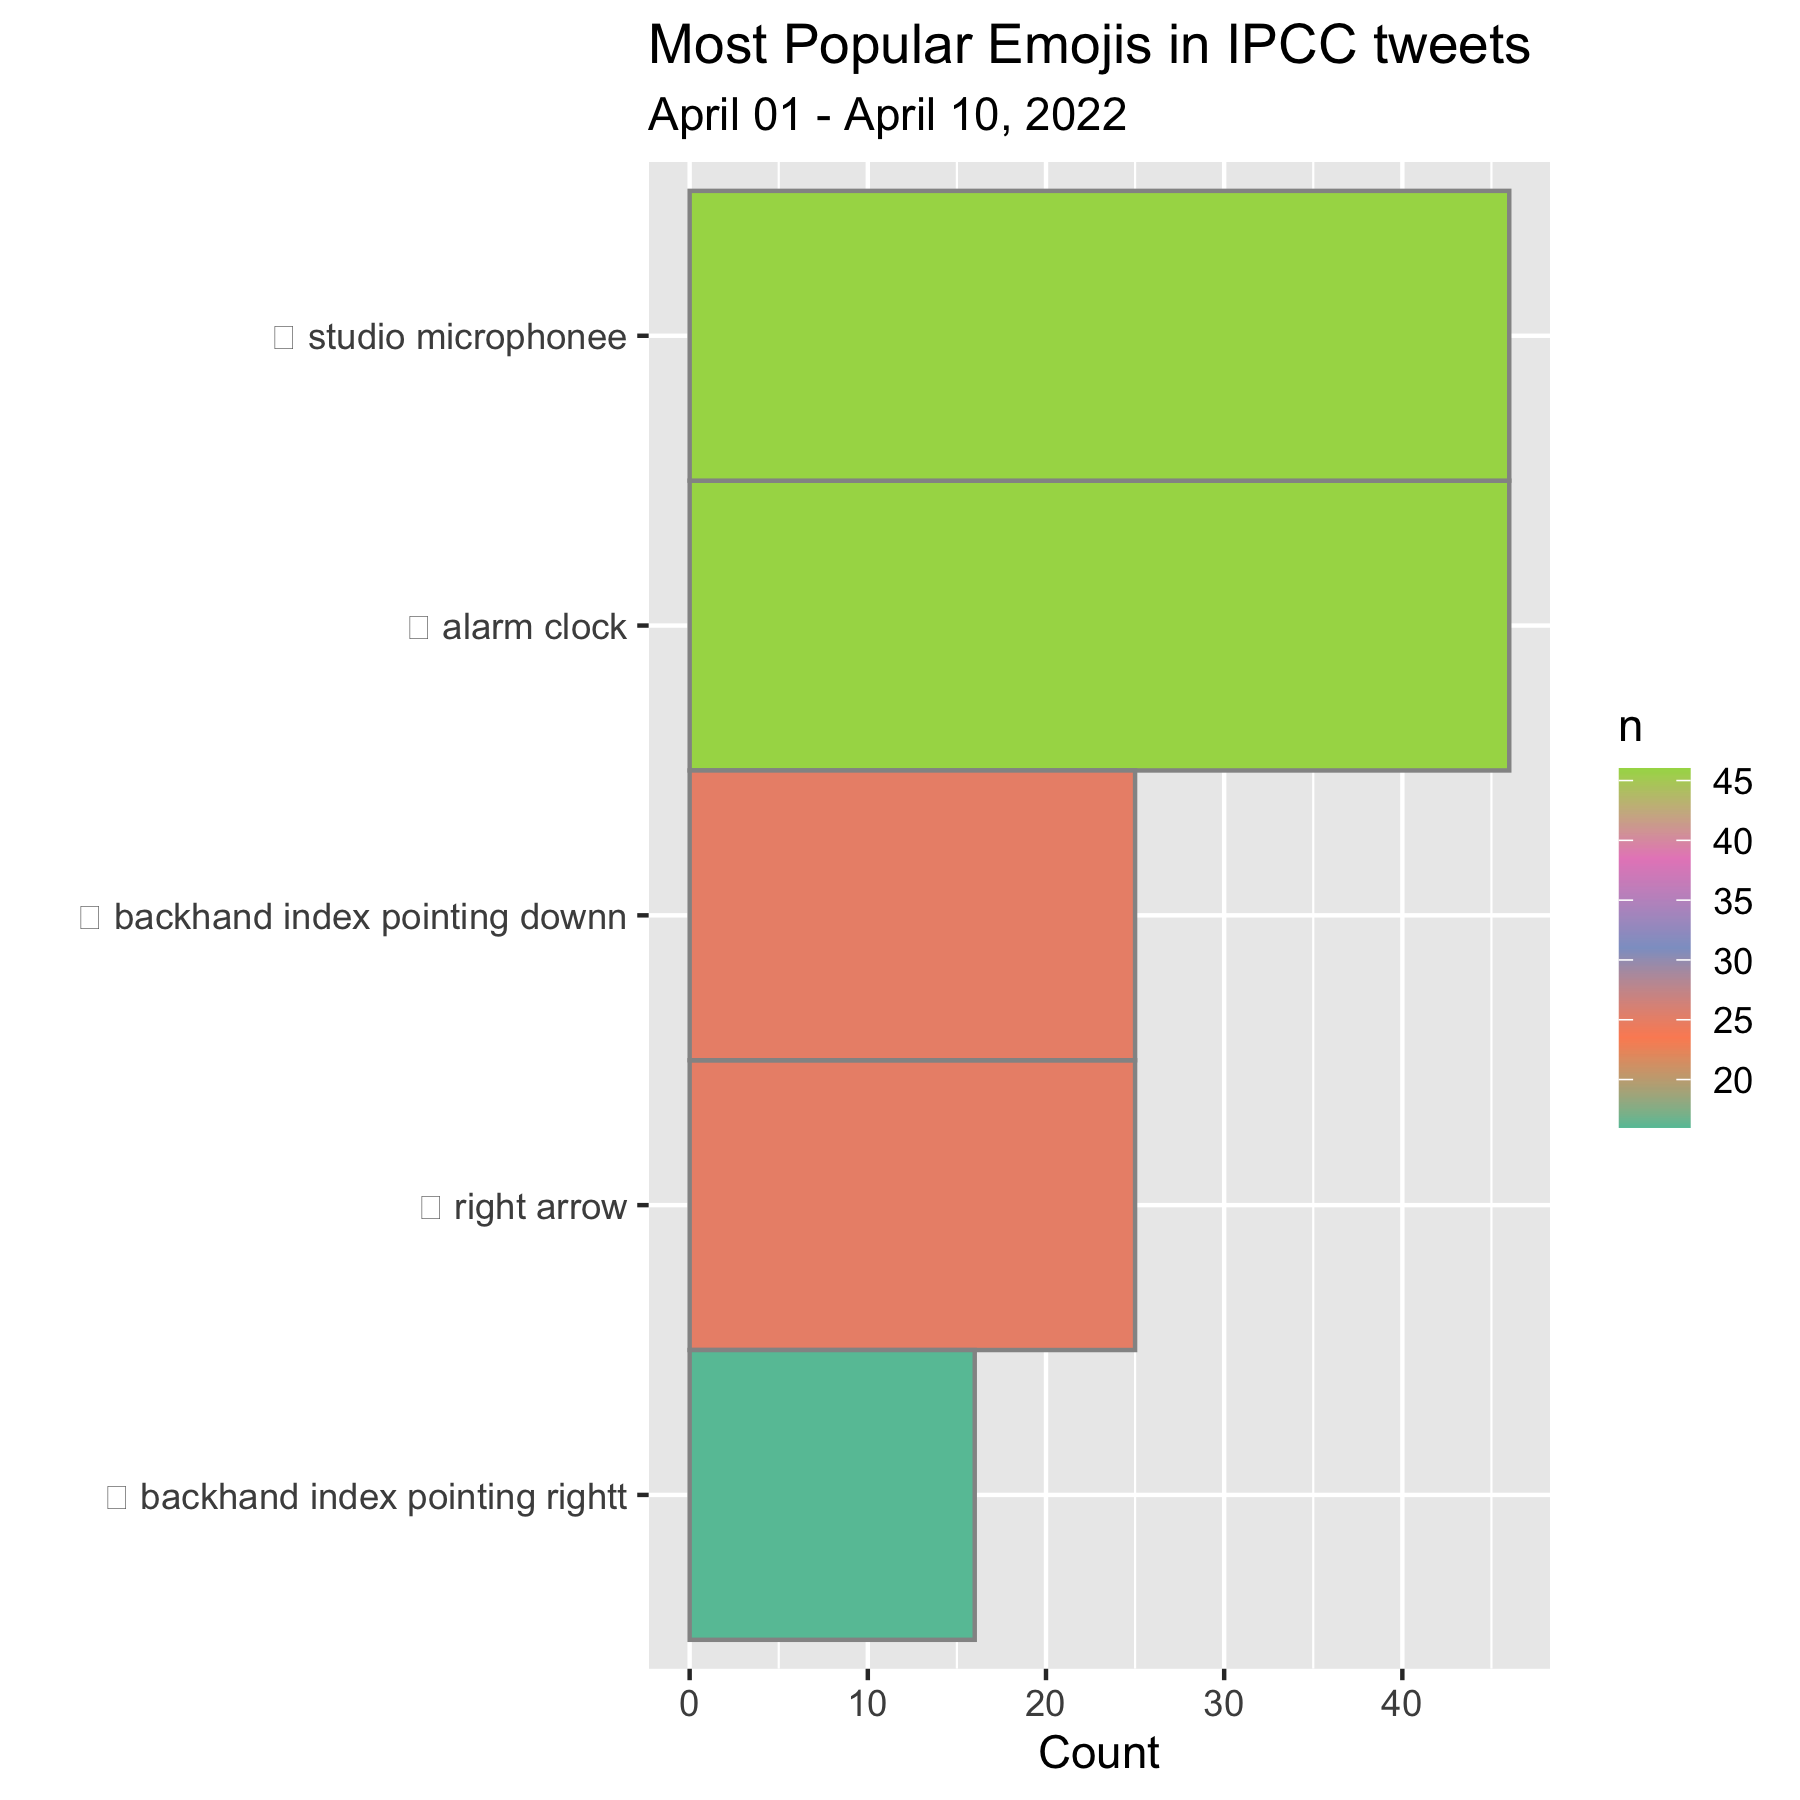
\includegraphics[totalheight=60mm,clip=true,viewport=0 0 500 300]{emojiplot.png}
 \end{frame}
 \end{document}

\end{document}
